\documentclass[a4paper,12pt]{article}

% --- Paketit ---
\usepackage[utf8]{inputenc}
\usepackage[T1]{fontenc}
\usepackage[finnish]{babel}
\usepackage{geometry}
\geometry{left=2.5cm, right=2.5cm, top=2.5cm, bottom=2.5cm}
\usepackage{amsmath, amssymb}
\usepackage{graphicx}
\usepackage{setspace}
\usepackage{xcolor}


% --- Koodilohkojen tyylit (Listings) ---
\usepackage{listings}
\definecolor{codegreen}{rgb}{0,0.6,0}
\definecolor{codegray}{rgb}{0.5,0.5,0.5}
\definecolor{codepurple}{rgb}{0.58,0,0.82}
\definecolor{backcolour}{rgb}{0.95,0.95,0.92}

\lstdefinestyle{mystyle}{
    backgroundcolor=\color{backcolour},   
    commentstyle=\color{codegreen},
    keywordstyle=\color{magenta},
    numberstyle=\tiny\color{codegray},
    stringstyle=\color{codepurple},
    basicstyle=\ttfamily\footnotesize,
    breakatwhitespace=false,         
    breaklines=true,                 
    captionpos=b,                    
    keepspaces=true,                 
    numbers=left,                    
    numbersep=5pt,                  
    showspaces=false,                
    showstringspaces=false,
    showtabs=false,                  
    tabsize=2
}
\lstset{style=mystyle}

% --- Kaaviot (TikZ) ---
\usepackage{tikz}
\usetikzlibrary{shapes.geometric, arrows, positioning}

% --- Otsikointi ---
\title{Resurssien optimointisimulaattorin toteutussuunnitelma}
\author{Elias Ervamaa}
\date{\today}

% --- Otsikoiden muotoilu ---
\usepackage{titlesec}

% Section (Pääotsikko): Muutetaan \Huge -> \Large (hieman isompi kuin leipäteksti)
\titleformat{\section}
  {\normalfont\large\bfseries} % Tyyli: Large fontti, Bold
  {\thesection}                % Numerointi (esim. "1")
  {1em}                        % Väli numeron ja tekstin välissä
  {}

% Subsection (Alaotsikko): Muutetaan \Large -> \large (vain vähän isompi)
\titleformat{\subsection}
  {\normalfont\normalsize\bfseries}
  {\thesubsection}
  {1em}
  {}

\begin{document}

\maketitle

\section{Johdanto}
Tämä dokumentti kuvaa teknisen arkkitehtuurin ja toteutuksen vakuutusyhtiön resurssien allokointiongelman ratkaisemiseksi. Tavoitteena on validoida matemaattisesti johdettu optimointimalli käyttämällä data-vetoista lähestymistapaa. \\

Toteutus ei nojaa ennalta annettuihin parametreihin, vaan simuloi todellista Data Science -prosessia, jossa mallin syötteet on ensin louhittava raakadatasta SQL-kyselyillä.



\newpage
\section{Järjestelmäarkkitehtuuri}

Ratkaisu koostuu kolmesta itsenäisestä moduulista, jotka muodostavat jalostusputken.

\begin{center}
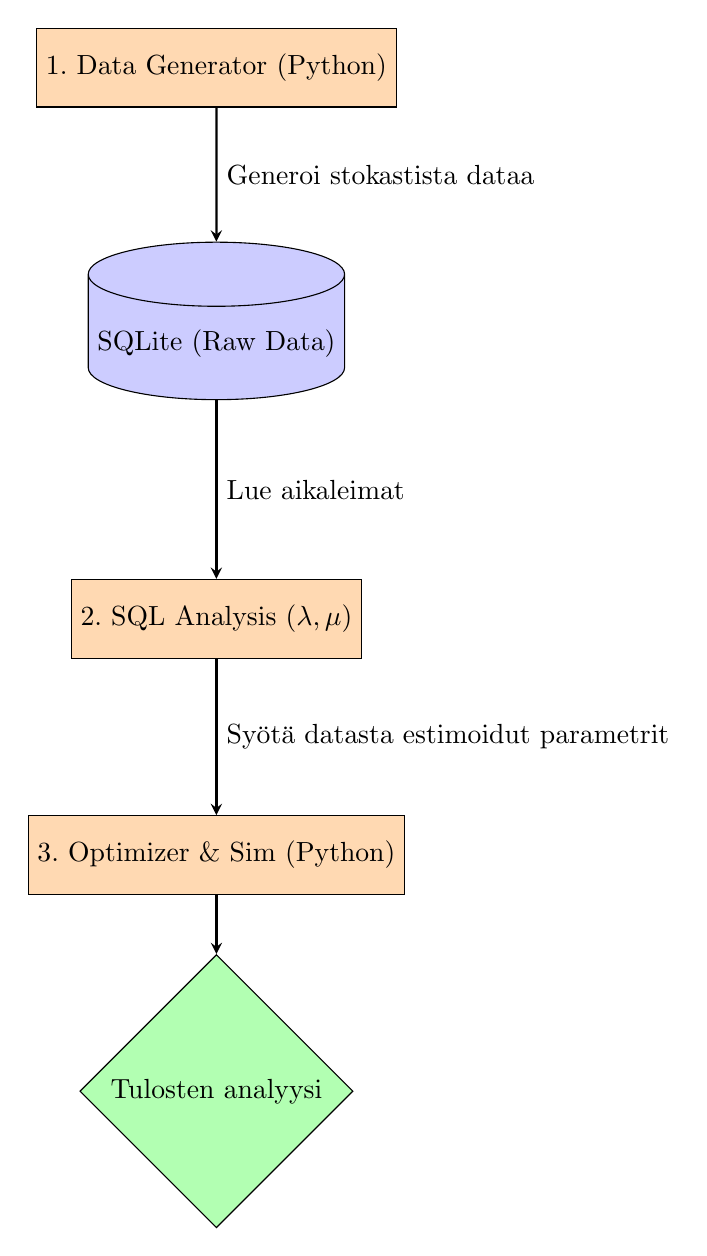
\begin{tikzpicture}[node distance=2cm]
    % Tyylit
    \tikzstyle{process} = [rectangle, minimum width=3cm, minimum height=1cm, text centered, draw=black, fill=orange!30]
    \tikzstyle{database} = [cylinder, shape border rotate=90, draw, minimum height=2cm, minimum width=1.5cm, aspect=0.25, fill=blue!20, text centered]
    \tikzstyle{decision} = [diamond, minimum width=3cm, minimum height=1cm, text centered, draw=black, fill=green!30]
    \tikzstyle{arrow} = [thick,->,>=stealth]

    % Solmut
    \node (gen) [process] {1. Data Generator (Python)};
    \node (db) [database, below of=gen, yshift=-1.5cm] {SQLite (Raw Data)};
    \node (sql) [process, below of=db, yshift=-1.5cm] {2. SQL Analysis ($\lambda, \mu$)};
    \node (sim) [process, below of=sql, yshift=-1cm] {3. Optimizer \& Sim (Python)};
    \node (out) [decision, below of=sim, yshift=-1cm] {Tulosten analyysi};

    % Nuolet
    \draw [arrow] (gen) -- node[anchor=west] {Generoi stokastista dataa} (db);
    \draw [arrow] (db) -- node[anchor=west] {Lue aikaleimat} (sql);
    \draw [arrow] (sql) -- node[anchor=west] {Syötä datasta estimoidut parametrit} (sim);
    \draw [arrow] (sim) -- (out);
\end{tikzpicture}
\end{center}

\subsection{Moduulien kuvaus}
\begin{enumerate}
    \item Generoi synteettistä vakuutusdataa piilotetuilla parametreilla. Tämä simuloi reaalimaailman ilmiötä, jonka lainalaisuudet ovat tuntemattomia.
    \item Toimii analyytikon roolissa. Lukee raakadatan tietokannasta ja estimoi saapumis- ja palveluprosessien parametrit ($\lambda, \mu$) SQL-aggregaatioilla.
    \item Laskee teoreettisen optimin estimoitujen parametrien perusteella ja suorittaa diskreettitapahtumasimulaation (DES) verifioidakseen tuloksen.
\end{enumerate}




\newpage
\section{Tietokantasuunnittelu}
Datavarastona käytetään SQLite-relaatiotietokantaa. Skeema on suunniteltu tallentamaan tapahtumatason dataa, josta prosessimittarit voidaan johtaa.

Taulu \texttt{vakuutustapahtumat}:
\begin{lstlisting}[language=SQL]
CREATE TABLE vakuutustapahtumat (
    id INTEGER PRIMARY KEY AUTOINCREMENT,
    vahinkotyyppi TEXT,    -- 'henkilo' tai 'auto'
    saapumisaika REAL,     -- Aikaleima (t)
    kasittely_alkoi REAL,  -- Aikaleima (t)
    kasittely_paattyi REAL -- Aikaleima (t)
);
\end{lstlisting}




\section{Parametrien estimointi}
\subsection{Saapumisintensiteetti ($\lambda$)}
Poisson-prosessin intensiteetti lasketaan jakamalla havaintojen määrä havaintoajan pituudella.

\begin{lstlisting}[language=SQL]
--Lasketaan lambda (tapahtumaa per aikayksikko)
SELECT 
    vahinkotyyppi,
    COUNT(*) * 1.0 / (MAX(saapumisaika) - MIN(saapumisaika)) as lambda_est
FROM vakuutustapahtumat
GROUP BY vahinkotyyppi;
\end{lstlisting}

\subsection{Palvelunopeus ($\mu$)}
Palvelunopeus on keskimääräisen palveluajan käänteisluku ($\mu = 1 / E[S]$). SQL:ssä laskemme ensin palvelun keston erotuksena \texttt{paattyi - alkoi}.

\begin{lstlisting}[language=SQL]
-- Lasketaan mu (palvelunopeus)
SELECT 
    vahinkotyyppi,
    1.0 / AVG(kasittely_paattyi - kasittely_alkoi) as mu_est
FROM vakuutustapahtumat
GROUP BY vahinkotyyppi;
\end{lstlisting}




\newpage
\section{Diskreettitapahtumasimulaatio}

Simulaattori on toteutettu Pythonilla ilman ulkoisia kirjastoja.

Simulaatio noudattaa johdetun matemaattisen mallin oletusta (Skaalattu M/M/1), jossa resurssimäärä $x$ mallinnetaan palvelukapasiteetin kasvuna. Systeemi toimii kuten yksi "superpalvelija", jonka työskentelynopeus on $x$-kertainen yksittäiseen työntekijään verrattuna.

\subsection{Toimintaperiaate}
Simulaatio etenee tapahtumapohjaisesti. Aikajana ei ole jatkuva, vaan simulaatiokello hyppää aina suoraan seuraavan tapahtuman aikaleimaan.

Järjestelmän tilaa seurataan seuraavilla komponenteilla:
\begin{itemize}
    \item \textbf{Tapahtumakalenteri:} Aikajärjestyksessä oleva lista tulevista tapahtumista. Tyypit ovat \textit{SAAPUMINEN} ja \textit{POISTUMINEN}.
    \item \textbf{Tilamuuttujat:}
    \begin{itemize}
        \item \textit{Palvelijan tila:} Vapaa (0) tai Varattu (1).
        \item \textit{Jonon pituus:} $L(t)$.
    \end{itemize}
    \item \textbf{Suorituskykymittarit:} Muuttujat, joihin kerätään dataa keskiarvojen laskemista varten (esim. \textit{kumulatiivinen odotusaika} ja \textit{palveltujen asiakkaiden lkm}).
\end{itemize}



\subsection{Algoritmi}
Simulaatiosilmukka toimii seuraavalla logiikalla, kunnes asetettu simulointiaika $T_{max}$ täyttyy. Olkoon $x$ resurssien määrä (kokonaisluku).

\begin{enumerate}
    \item Asetetaan kello $t=0$ ja luodaan ensimmäinen SAAPUMINEN-tapahtuma kalenteriin.
    
    \item \textbf{Pääsilmukka:}
    \begin{enumerate}
        \item \textbf{Kellon siirto:} Otetaan kalenterista tapahtuma, jolla on pienin aikaleima, ja siirretään kello $t$ tähän aikaan.
        
        \item \textbf{Jos tapahtuma on SAAPUMINEN:}
        \begin{itemize}
            \item Luodaan seuraava saapumisaika (Poisson-prosessi, intensiteetti $\lambda$) ja lisätään se kalenteriin.
            \item Jos palvelija on vapaa:
            \begin{itemize}
                \item Asiakas pääsee palveluun.
                \item Arvotaan palveluaika $S$. Huom: Koska käytössä on $x$ resurssia, palvelunopeus on $x \cdot \mu$. Tällöin $S \sim \text{Exp}(x\mu)$.
                \item Luodaan kalenteriin tapahtuma \textit{POISTUMINEN} ajalle $t + S$.
                \item Asetetaan palvelija varatuksi.
            \end{itemize}
            \item Jos palvelija on varattu:
            \begin{itemize}
                \item Lisätään asiakas odotusjonoon.
            \end{itemize}
        \end{itemize}
        
        \item \textbf{Jos tapahtuma on POISTUMINEN:}
        \begin{itemize}
            \item Asiakas poistuu järjestelmästä.
            \item Jos odotusjonossa on asiakkaita:
            \begin{itemize}
                \item Otetaan seuraava asiakas jonosta.
                \item Arvotaan palveluaika $S \sim \text{Exp}(x\mu)$.
                \item Luodaan kalenteriin uusi \textit{POISTUMINEN} ajalle $t + S$.
                \item Palvelija pysyy varattuna.
            \end{itemize}
            \item Jos jono on tyhjä:
            \begin{itemize}
                \item Asetetaan palvelija vapaaksi.
            \end{itemize}
        \end{itemize}
    \end{enumerate}
\end{enumerate}

\subsection{Optimointihaku (Grid Search)}
Simulaattori ajaa yllä kuvattua algoritmia iteratiivisesti. Koska teoreettinen ratkaisu $x^*$ on jatkuva luku, simulaattori testaa $x^*$:n ympärillä olevat kokonaislukuparit $(x_1, x_2)$, jotka toteuttavat budjettirajoitteen. Näin löydetään paras mahdollinen diskreetti allokaatio.

\end{document}